In the previous chapters, we focused on a nonlinear mechanism by which the system can shift from on state to another by changing an external parameter (the bathymetry) in a deterministic manner.


%a system might display extreme evens, in particular how to develop reduced models that allow us to gain insight on how nonlinearity plays a role in the modulation of wave packets in surface gravity waves.

In this chapter, we will focus on another  problem specific to nonlinear systems: the prediction of regime  changes.

Dynamical systems can, not only change their stability or periodicity, but they can also have the property of having several stable states (attractors) which can coexist for a given set of parameters and/or forcings.
This property is referred as multi-stability; which means a system might also change, or flip, state between multi-stable solutions.

The field of early warning signals (EWS) studies the methods to predict systems going through sudden changes in behavior when they change from one state to another.
A system abruptly changes its behavior, due to a small change in some parameter. 

One of the ways in which a system can move from one stable state to another is trough a critical transition. 
\Cref{fig: stability_example} exemplifies this effect with a system where a change of sign of the parameter $\la$ changes abruptly the stable solutions of the system.  Therefore, any small change in the parameter that leads to a change of sign has big implications for the state of the system. 



\begin{figure}[htb]
	\begin{center}
		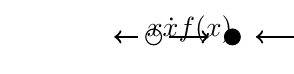
\begin{tikzpicture}
			\tzaxes(-2,-2)(2,2){$x$}{$\dot{x}$}
			\tzfn[col2,thick]{(\x)*(\x-1)*(\x+1)}[-1.5:1.5]{$f(x)$}[ar]
			\draw [->,thick](0.8,0) -- (0.3,0);
			\draw [->,thick](-0.8,0) -- (-0.3,0);
			\draw [->,thick](1.2,0) -- (1.5,0);
			\draw [->,thick](-1.2,0) -- (-1.5,0);
			\node (a) at (0,0) {};
			\filldraw (a.center) circle [radius=0.1cm];
			\draw (a)+(1,0) circle [radius=0.1cm];
			\draw (a)+(-1,0) circle [radius=0.1cm];
		\end{tikzpicture}  \qquad \qquad
		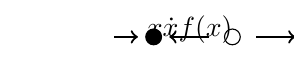
\begin{tikzpicture}
			\tzaxes(-2,-2)(2,2){$x$}{$\dot{x}$}
			\tzfn[col2,thick]{-(\x)*(\x-1)*(\x+1)}[-1.5:1.5]{$f(x)$}[ar]
			\draw [->,thick](0.3,0) -- (0.8,0);
			\draw [->,thick](-0.3,0) -- (-0.8,0) ;
			\draw [->,thick](1.5,0) -- (1.2,0) ;
			\draw [->,thick](-1.5,0) -- (-1.2,0) ;
			\node (a) at (0,0) {};
			%	\node[circle,draw,minimum size=10cm] (a) at (0,0) {};
			\draw (a.center) circle [radius=0.1cm];
			\filldraw (a)+(1,0) circle [radius=0.1cm];
			\filldraw (a)+(-1,0) circle [radius=0.1cm];
			%	\tzfn'[red,thick]{(\x)^2}[-1:2]{$f^{-1}(x)$}\\[ar] % inverse
		\end{tikzpicture}
	\end{center}
	\caption{Stability of $\dot{x}=\lambda (x+1)x(x-1)$. If $\lambda >0$(left) then the only stable solution is $x=0$; for $\la<0$(right) the system has two stable solutions $x={-1,1}$. $\la=0$ marks a critical transition for this system.}
	\label{fig: stability_example}
\end{figure}



Tipping points have been identified or are suspected in many systems, from climate \citep{Cai2016,Lenton2011,Boers2017}, phase transitions \citep{Fullsack2022}, fluid dynamics \citep{Lucarini2014,Yang2021}, to seizures \citep{no_cls_epileptic}, population dynamics \citep{10.1086/681573,Bathiany2016} as exemplified in (\cref{fig: climate_bistability}), social dynamics \citep{SCHEFFER2020a}, disease outbreaks \citep{doi:10.1098/rsbl.2019.0713}, cell-death \citep{Sarkar2019}.



\begin{figure}[bhtp]
	\centering
	\includegraphics[width=0.4\columnwidth]{Images/Metrics/sahel_multistable}
	\caption{Stability landscape of the Green Sahara and desert. The larger the atmosphere–vegetation feedback (i.e. moving towards the lower left of the figure), the sharper the transition between the two states. (Modified from Model Calendar 2015, designed by Elsa Wikander at Azote, funded by the Beijer Institute of Ecological Economics and the Stockholm Resilience Centre.) Taken from \cite{Bathiany2016}.}
	%	\caption{Events per ms}
	\label{fig: climate_bistability}
\end{figure}



%To provide an early warning to such transitions, dynamical approaches have been proposed, in particular critical-slowing-down  \cite{Scheffer2009,Scheffer344,doi:10.1111/j.1600-0706.2012.20838.x}. However these dynamical approaches impose to observe the system evolution over time after a perturbation. 

%
%%%% this can go somewhere else %%%%           

%Predicting this transitions can be very challenging, in real systems it is often difficult to distinguish between bi-stable and abrupt transition situations, where the noise blurs the observed phase diagram. 
%However, in both cases the management of technical, human or natural systems calls for EWS for the transition.
